%! Author = Administrator
%! Date = 2021/7/2

\chapter{概要设计}
本章主要是在需求分析的基础上,对该云服务的整体架构以及各个模块的设计进行详尽的阐述,在本章节的基础上,可以从总体上了解设计思路,与后续具体实现打下坚实的基础。
该部分对需求进行具体的梳理,划分出各个功能模块和整体的系统架构。包括各个模块之间的数据流转、相互协作等。通过该部分的概要设计,可以为具体的系统实现提供工程上的依据和铺垫。


\section{系统整体结构}

\begin{figure}[H]
    \centering
    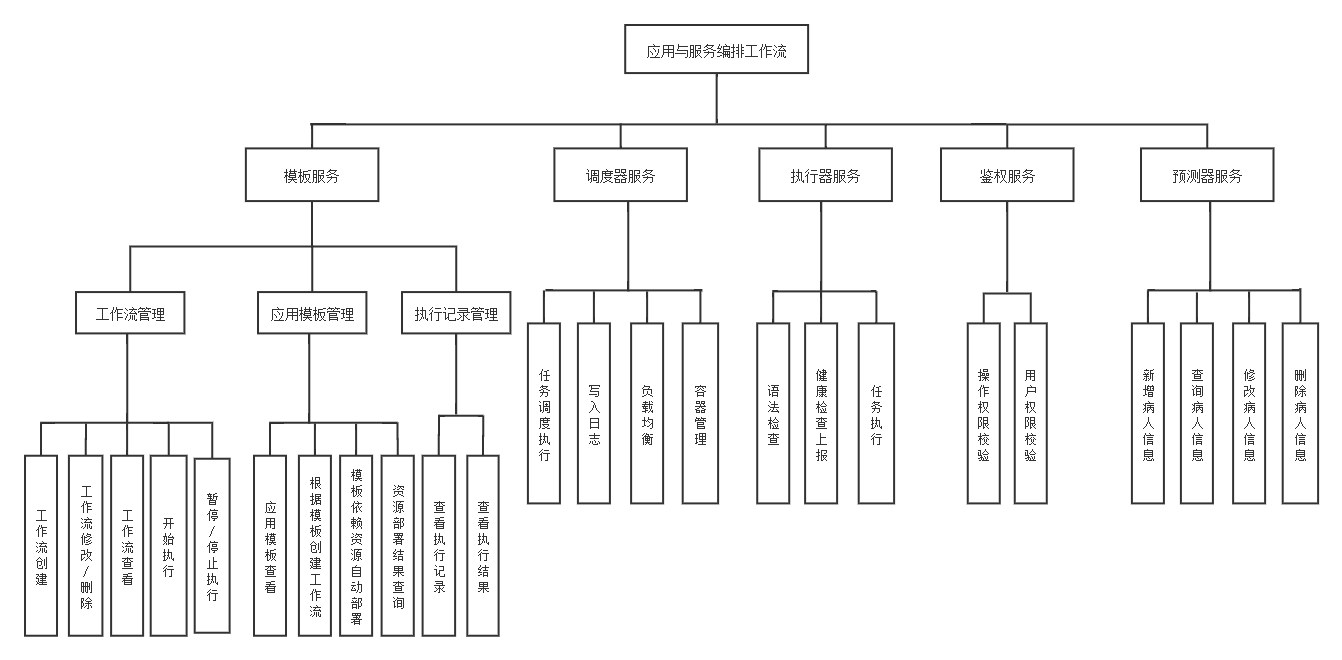
\includegraphics[width=1.0\textwidth]{sys_structure.png}
    \caption{系统整体架构图}
    \label{fig:系统整体架构图}
    \note{}
\end{figure}



如图所示,系统划分为5个微服务模块,分别是模板服务、调度器服务、执行器服务、鉴权服务和预测器服务,彼此之间通过RPC通信。

微服务依业务模块功能设计,以全自动的方式部署,与其他服务使用HTTP协议通讯,同时可使用最小规模的集中管理能力。\cite{jywfbpxt}
每个微服务仅关注于完成一件任务并很好地完成该任务。在所有情况下,每个任务代表着一个小的业务能力。尽管微服务这种架构风格没有精确的定义,
但其具有一些共同的特性,如围绕业务能力组织服务、自动化部署、对语言及数据的去集中化控制等。\cite{wlfwyh}

这样的设计目的是为了解耦用户界面的操作和后台执行服务。
模板服务提供的功能特点是类目众多,业务逻辑复杂;其余服务则是功能较为单一,业务逻辑清晰,但需要高性能高并发性,是数据密集型的微服务模块。

模板服务主要提供工作流相关的管理功能,包括普通工作流,模板工作流,工作流执行记录查询等。

调度器服务则提供模板服务所需要的接口功能,负责接收从模板服务发来的工作流执行请求,管理容器节点,负责执行工作流的前置准备工作和后置工作,包括日志处理、错误处理等。

鉴权服务提供用户权限的校验和申请功能,所有微服务模块的功能都需要或多或少的权限需求,因此,也是访问量较大的一个模块。

预测器服务提供对执行记录的管理,执行器的预测执行模式会调用此模块,根据历史执行行为记录,分支执行走向记录,进行节点执行的预测,尝试并行化此次执行。
并且在每次执行成功后,也会调用该模块进行记录数据保存。


\begin{figure}[H]
    \centering
    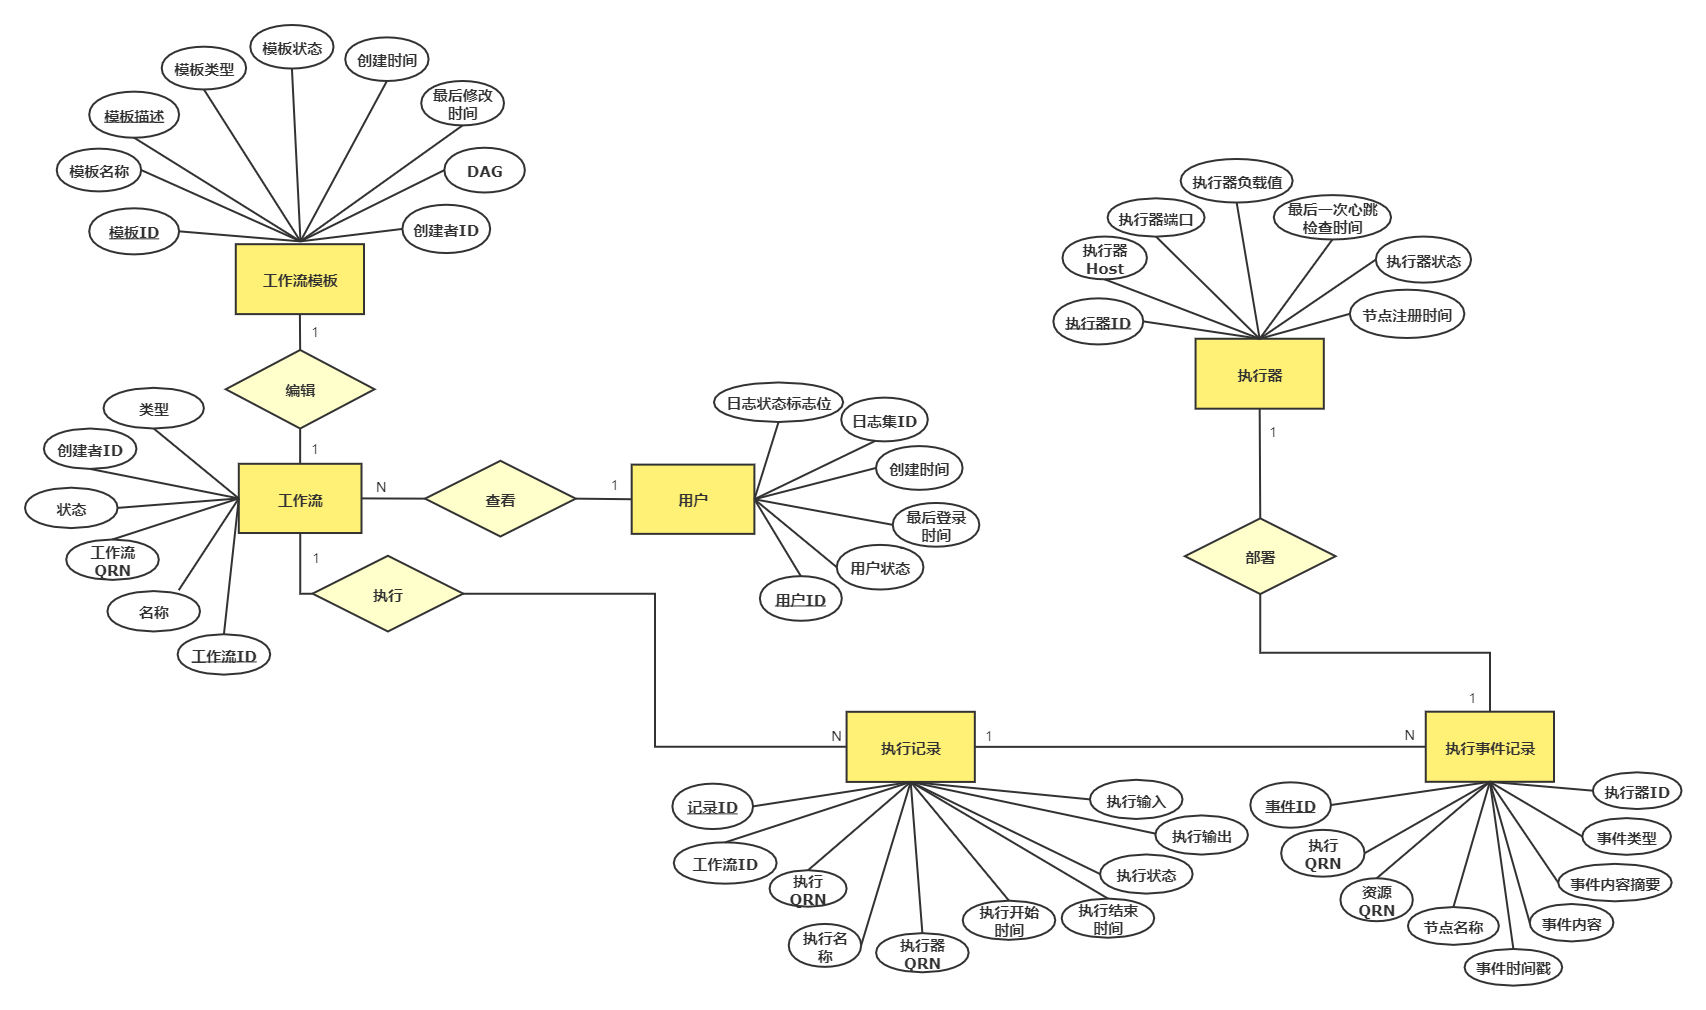
\includegraphics[width=1.0\textwidth]{er-1.png}
    \caption{ER关系图}
    \label{fig:ER关系图}
    \note{}
\end{figure}

如图4.2,根据划分的微服务模型梳理的所有数据流转的对象主要有工作流、工作流模板、执行记录、执行器。由上述的对象构建一个系统的模型。

首先,工作流是系统主要的操作对象。需要区分地,由于工作流对象较为复杂,故将其抽象成两个部分,由工作流对象本身存储轻量的数据,再以外键的形式连接
对应一个工作流模板对象,两者是一一对应的关系,这样一来,读取工作流对象时,不一定需要读取全量的数据,比如读取工作流状态时,不需要扫描那些数据量
可能非常大的列,比如图中工作流模板的DAG字段。

其次,工作流执行作为系统主要功能,其需要对用户展现的就是执行结果,而不是执行过程,因此,需要单独抽象出执行记录的对象概念,这个对象主要负责管理
每一个工作流的每一次执行。由于工作流通常具有多个任务节点,所以执行记录的每一行都可能对应多个任务节点。执行事件记录对象是每一个节点的执行记录,其
一个事件即代表一个工作流节点的执行结果,对于一个工作流来说,每个节点的结果是“过程”,而事件的总和,就是对应一个执行记录对象。

最后,执行器作为工作流执行的关键部件,需要维护一个执行器的注册表,这个表的对象就是每一个可用的执行器以及目前执行器的负载情况,确保每一次执行都是
可追溯的。

\section{功能模块设计}
考虑到设计并行执行器所影响的上下游,包括调度器服务、模板服务的架构仅适用于顺序执行器,需要对其一并进行兼容改造。因此按微服务模块划分
后的情况来展开叙述。


\subsection{模板微服务模块概要设计}

用户API层,提供对外服务的基础功能API,包括工作流的创建、修改、删除,DAG的编译与渲染显示等。将模板单独拆分为一个微服务的目的是为了尽量最小化调度执
行器的功能,使得调用量大的StartExecution接口并发能力提高。因此抽象出“工作流”对象,该模块所包含的功能都是以这个抽象对象为基础的,
由于普通用户对工作流进行的操作是低频的,因此该模块相对其它模块来说,是对性能要求更低的一个模块。

该服务直接提供对外的用户交互API,提供基于用户状态机列表、创建、更新、执行、删除等接口。由于原架构初始设计时未考虑到并发量大的场景,
导致对数据库进行了频繁的查询操作,由此导致了接口的QPS不高。改进方案是将数据库操作优化,3个查询可以合并为一个join查询,减少查询次数,
减少查询耗时。只查询需要的字段, 其他无用字段不写入select中, 优化网络流量。

由于原架构中的组件模块和消费者模块在数据量过大时存在性能瓶颈问题,在此次设计中不保留原设计包含的两个微服务模块,将组件服务合并入模板
服务,减少项目维护成本。同时去除消费者模块,转而将消费者模块所负责的消费任务交由专门的日志系统处理,而作为本系统则只需要提供编排调度
的服务,降低成本,这也符合服务设计单一职责的原则。这样一来,就可以通过更小的开销,异步地将调度执行结果持久化存储。以尽可能利用现有设施,
不引入新的复杂度。

以下是模块的概要设计分析:

\begin{figure}[H]
    \centering
    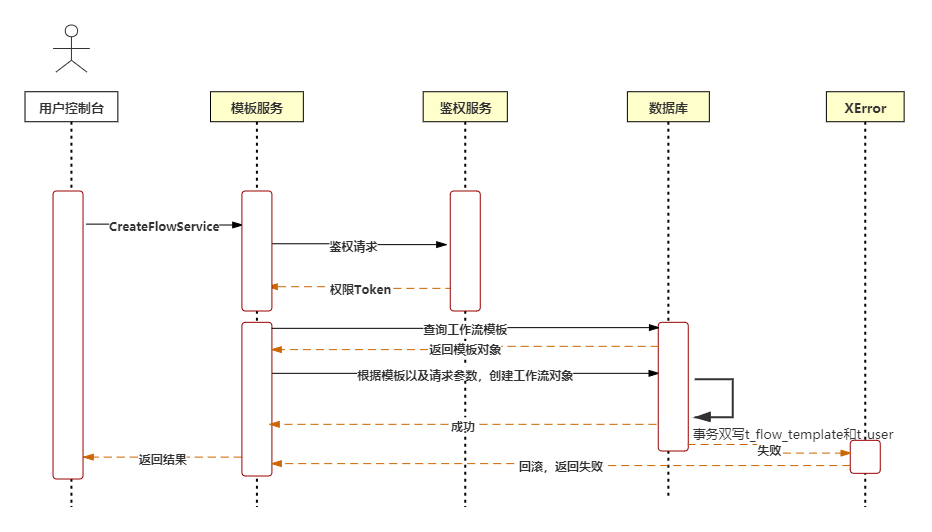
\includegraphics[width=1.0\textwidth]{create_flow_service.png}
    \caption{CreateFlowService时序图}
    \label{fig:CreateFlowService时序图}
    \note{}
\end{figure}

如上图4.3所示,工作流创建由CreateFlowService接口完成,涉及的服务主要是模板服务和鉴权服务。业务流程主要是先根据用户所设计的工作流,查询
其使用的工作流在模板表里的信息,再根据查询到的结果进行实际工作流的创建。每一次工作流的创建,都必须以一个模板为基础,这个模板可以是用户
自定义保存到数据库的,也可以是系统预设的简单示例模板,也可以是系统预设的具体业务场景的应用模板。


\begin{figure}[H]
    \centering
    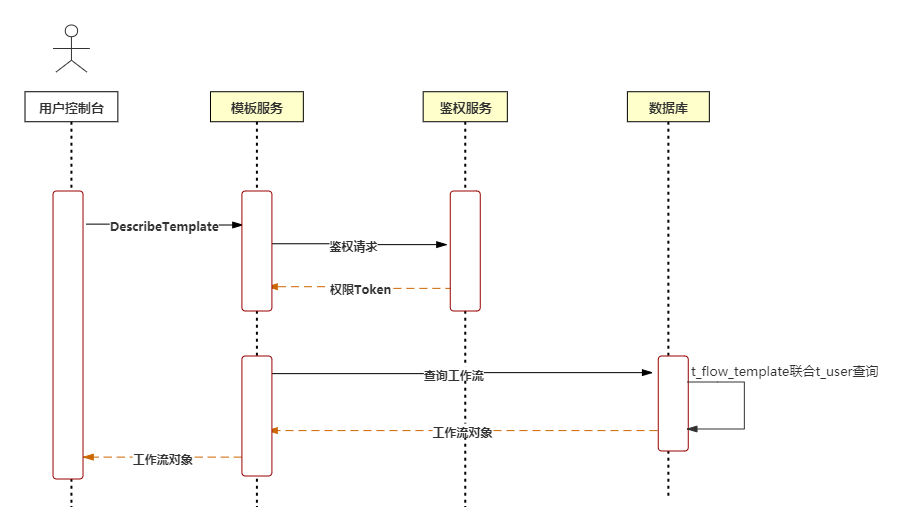
\includegraphics[width=1.0\textwidth]{describe_template.png}
    \caption{DescribeTemplate时序图}
    \label{fig:DescribeTemplate时序图}
    \note{}
\end{figure}

如上图4.4所示,工作流查询功能由DescribeTemplate对控制台提供,可以根据模板ID查询到用户对该模板是否拥有权限,如果有则返回该模板的信息。



\begin{figure}[H]
    \centering
    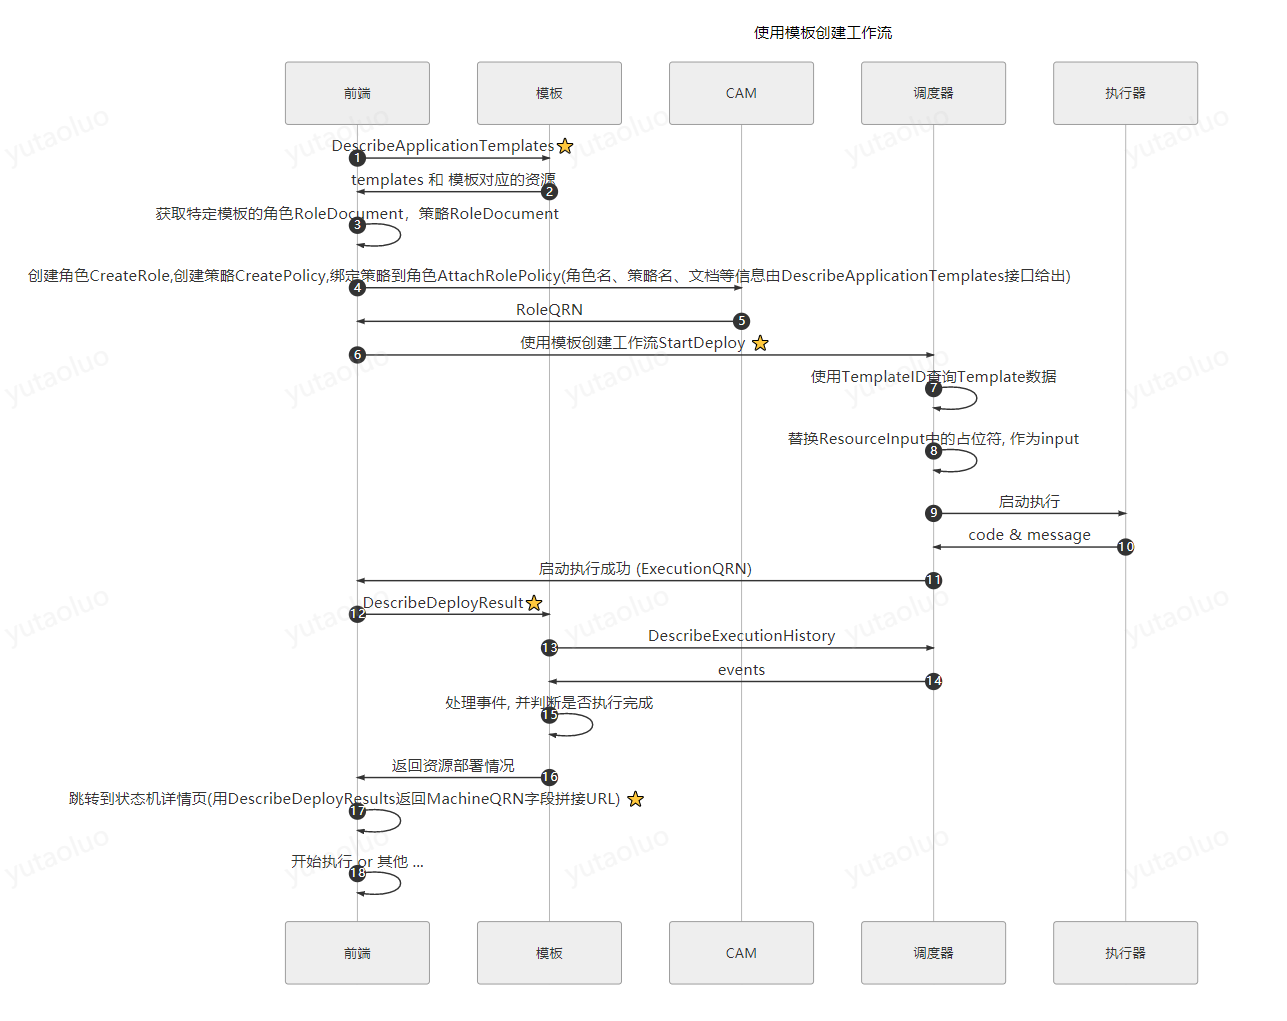
\includegraphics[width=1.0\textwidth]{app-template-sx-1.png}
    \caption{StartDeploy时序图}
    \label{fig:StartDeploy时序图}
\end{figure}
如上图4.5所示,应用模板的主要功能就是根据系统预设的应用模板去为用户创建一个相应的工作流。StartDeploy接口负责完成这样一项工作,
调用DescribeApplicationTemplates接口获取该应用模板所需的所有资源的创建策略JSON文档,用此文档到鉴权服务处申请对应云资源的权限。
资源创建完毕后,将执行命令提交到调度器,调度器会负责任务执行状态的管理,在成功执行后,会通知模板服务,此时通过DescribeDeployResults
接口就可以获取到最终的部署结果,如果成功,进行页面自动跳转,引导用户进入新创建工作流的页面。

\begin{figure}[h]
    \centering
    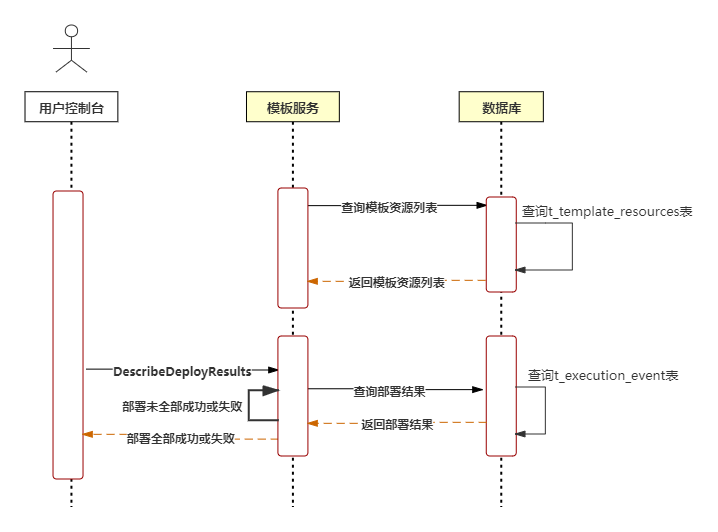
\includegraphics[width=0.8\textwidth]{describe_deploy_results.png}
    \caption{DescribeDeployResults时序图}
    \label{fig:DescribeDeployResults时序图}
\end{figure}
如上图4.6所示,应用模板的部署结果查询通过模板服务轮询DescribeDeployResults接口,直到全部返回结果都是确定状态(即成功或失败状态),或者
是查询次数到达上限,都会进行返回,通知用户此次部署的最终结果。

\subsection{调度器微服务模块概要设计}
调度器服务负责任务执行时的容器调度,执行记录生成投递等功能。在接收一个待执行的任务时,会向调用方返回一个ExecutionQrn,该字段是一个
资源定位符,用于唯一表示此次执行。

调度器服务模块在运行时划分为两个不同职责的微服务实例,实例类型之一负责接收模板服务传来的对状态机调度执行的请求,进行必要的选取执行器、保证负载均衡、执行初
始化、状态写库等操作;另一个类型是运行在消费者模式下,负责将执行完的节点日志写入数据库。之所以需要消费者模式的调度器,是由于数据库承载不了大量的写入,需要
使用消费者进行削峰填谷。

写执行历史记录到数据库:在3500万条数据的情况下,一个插入操作耗时约1000ms;而2700万数据量情况下, 一个insert耗时约10ms,MySQL的耗时在海
量数据下是非线性增长的。需要将日志中间件切换至Redis,以满足业务需要。

技术方案是,将日志接入云原生日志服务,只需要发送一个HTTP请求,这样一来,模板服务的请求在执行完后日志直接发送到对接的云日志服务CLS,
无需等待消费者消费信息,消除了性能瓶颈,降低了运行成本。


调度器模块负责根据容器的负载情况,读取数据库中的所有可用执行器节点IP,选取一个闲置的容器节点进行任务节点的执行。
流程大致分为如下几步:
\begin{enumerate}
    \item processor注册

    主要接口就是 ProcessorRegister,节点由执行器启动的时候进行注册;
    在自己消亡的时候,进行注销(同一个接口,参数 RegistrationType 区分。0,注册;1,注销)。
    注册过的 processor 会在数据库的t\_processor 表存一条记录。
    调度器在分发命令的时候,会从 t\_processor 找运行中的 processor ,即状态为 0 的 processor。

    对注册后的所有容器定期进行健康检查,所以容器的状态枚举值应包含如下几种情况:

    0:正常

    1:自主注销

    2:被动注销,即健康检查进行的强行注销

    \item 命令提交

    这里的命令提交,提交的是直接执行的请求。

    命令提交后, 先获取当前的template的TCSL,因为每一次执行,当前执行的template的TCSL是被存下来的。然后生成执行Qrn,
    尝试插入一条Execution数据,并判断是使用哪种执行器引擎,根据类型转发到指定的引擎。

    这种触发性的工作流,它的启动是异步的。当执行的时候,带过来参数和要执行的状态机的qrn
    name是这一次执行的name,用户可以自己传,如果不自己传,则系统创建一个StateMachineQrn,形如
    qrn:qcs:asw:sh:1300074211:http:json:flowmachine:flowservicetest:bcrlj428。
    \item 异常流检查和处理
    用于处理异常流程的是定时器healthyTimer,用于对容器实例的健康检查。
    \item 启动执行
    整体过程如下:
    用户编辑完成一个状态机后,需要启动这个状态机
    通过 StartExection 接口进行启动调度器来选择相应的引擎来执行。引擎执行完成后,将数据写进kafka。调度器对kafka进行消费,
    然后将数据写进 t\_execution\_event表。
    \item 开始部署应用模板(用于部署模板依赖的资源的模板)时, 和当前的状态机执行有些区别, 因此单独创建一个StartDeploy接口
    先获取应用资源模板(用来创建状态机依赖的资源的模板), 再组装请求(替换占位符内容, 拼接输入等)调用执行器开始部署。
    \item 停止执行
    在execution表中找到对应的调度器ip, 拼接请求(executionQRN, 停止命令)后, 发送RPC请求给到执行器. 再由执行器负责停止执行。
    \item 执行结果
    任务提交后,等待结果的返回,返回的数据是JSON标准输出。用户通过查询界面提供的标准输出,来获取结果。在后台,这些结果会被调度器模块存储到
    t\_execution\_event进行持久化管理,方便收集执行记录和定位问题。
\end{enumerate}

\begin{figure}[H]
\centering
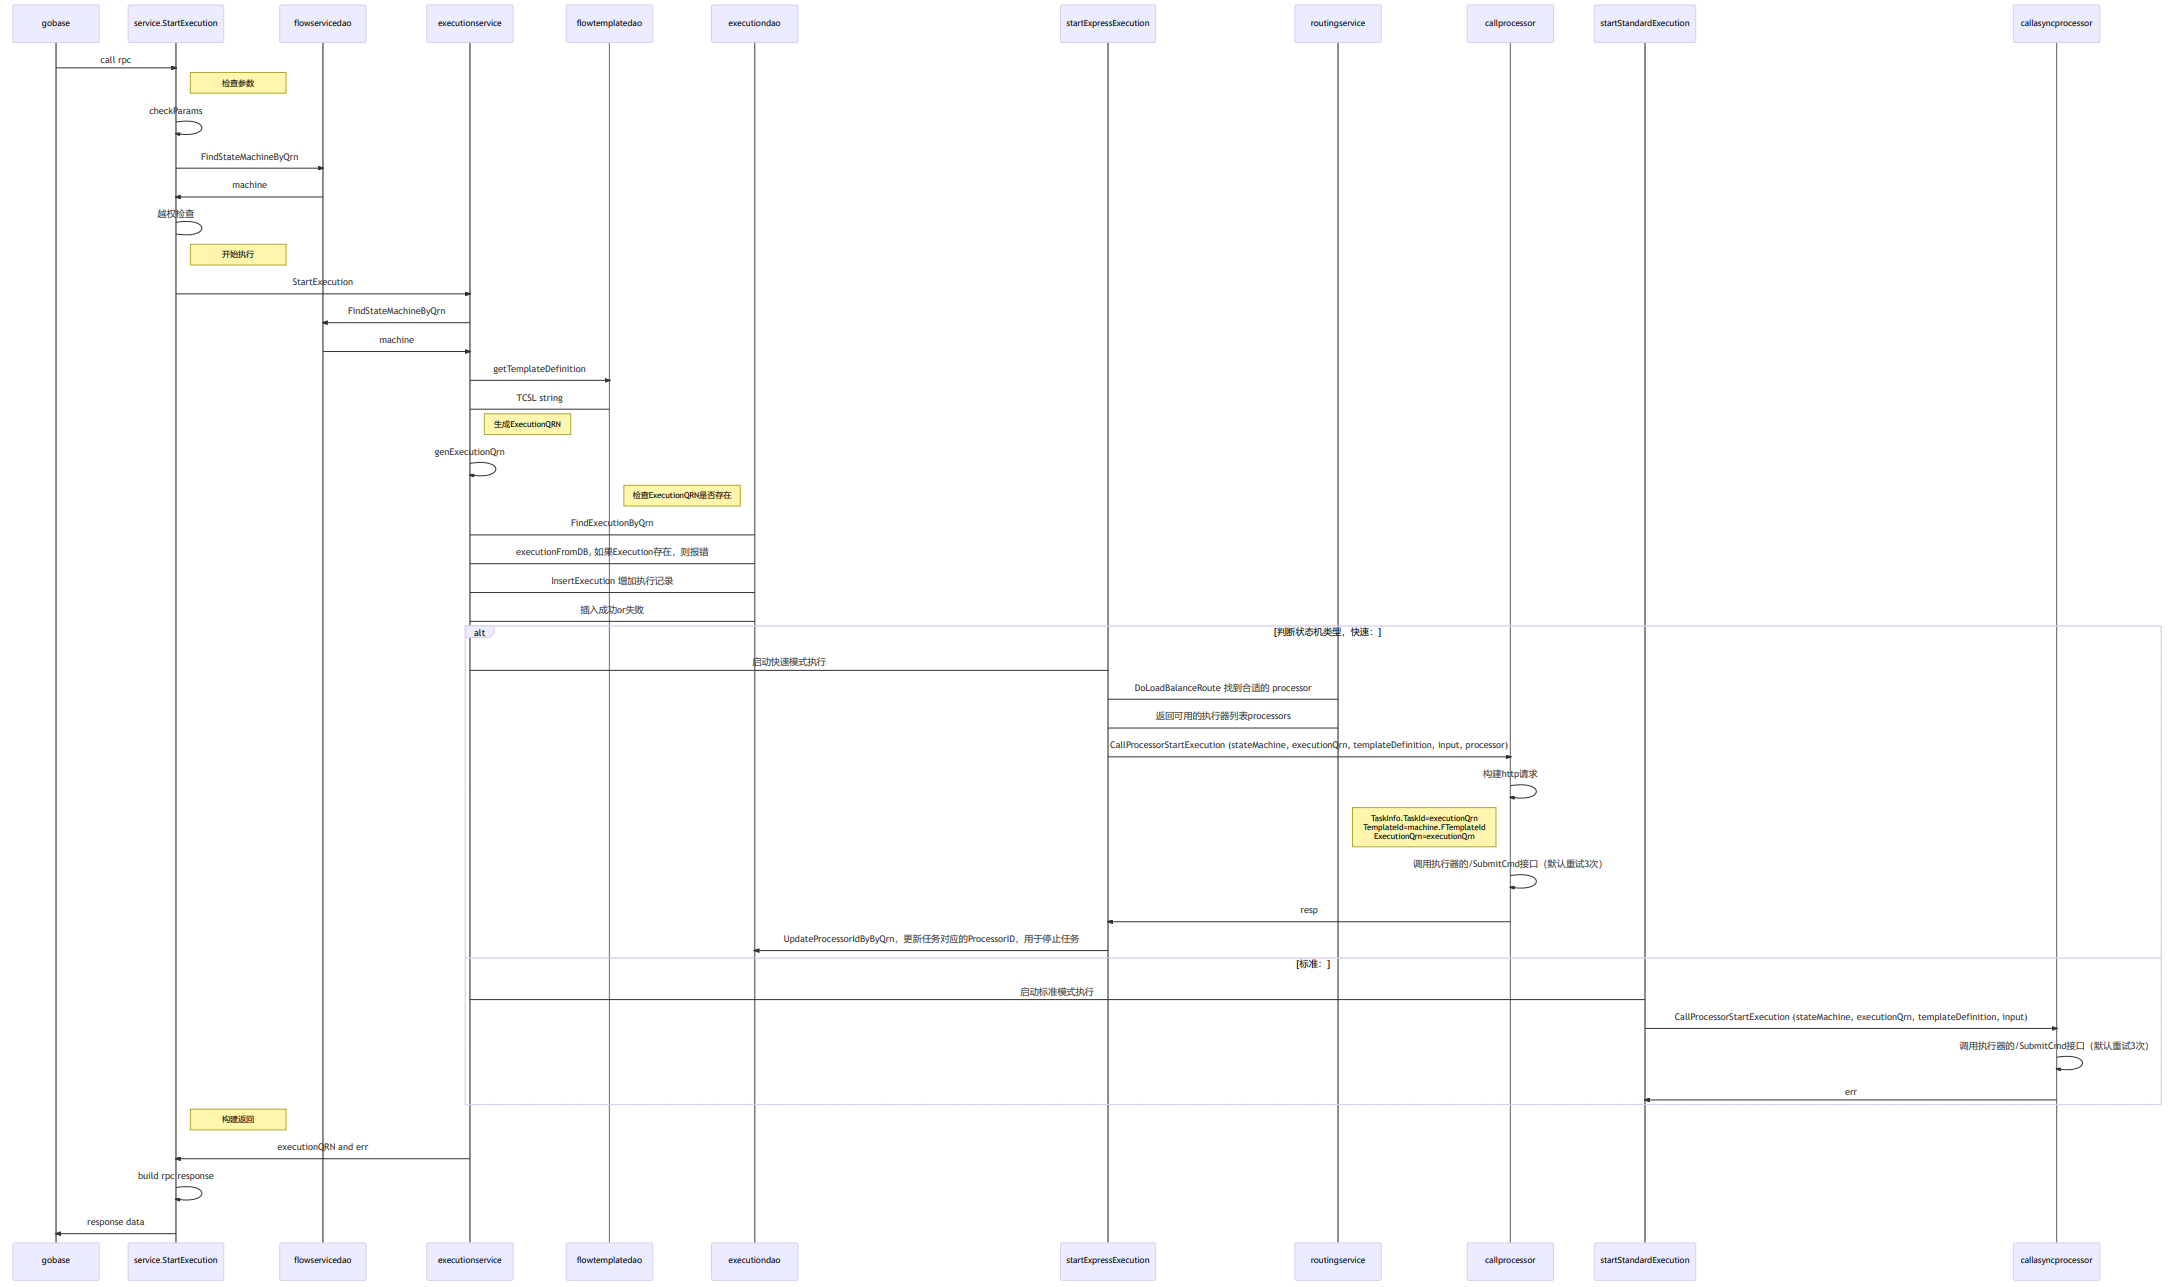
\includegraphics[width=1.0\textwidth]{start-execution-1.png}
\caption{开始执行}
\label{fig:kszx}
\end{figure}

如上图4.7所示,工作流开始执行功能是模板服务提供的主要功能之一。StartExecution接口负责提交执行任务到调度器。该接口业务逻辑复杂,
涉及到了大部分的微服务模块。 外部模块通过StartExecution接口访问调度器服务,调度器负责协调数据层和执行器引擎服务。根据执行方式的不同,有两种策略选择:

\begin{enumerate}
    \item 标准执行:不进行负载均衡,由执行器负责执行的流程。针对长时间运行、持久且可审计的工作流
    \item 快速执行:在之前注册上报的执行器信息和健康检查情况符合要求的表中查找执行器IP,通过负载情况计算出一个最合适的。针对大批量的事件处理工作负载。
\end{enumerate}


设计思路是优先保证引擎的高可扩展性,便于今后扩展需求时,不用再次改动引擎本身的架构,只要满足现有的条件:
\begin{itemize}
    \item 标准的输入,能被调度器调度
    \item 输出是标准的,能被消费
\end{itemize}

容器的健康检查机制和回收策略:
\subsubsection{容器健康检查机制}

如今,在分布式系统的设计之中,健康检查机制是必不可少的,它可以用于检查服务可用性,以免服务相互调用时出现异常。
对于Docker容器来说,由于容器的实体是一个进程,通过检查Docker进程就可以达到健康检查的目的\cite{zw1}。

在本系统中,由于需要让模板服务感知到执行任务的服务节点的存在,从而必须维护一个服务器列表缓存,因此也需要一个管理机制,来管理这个列表
状态的更新。

这里,通过参照Kubernetes提供的Liveness与Readness探针分别对Container及其服务健康状态进行检查的机制\cite{wfwr442},实现了执行器节点的健康检查。
每个可用执行节点会每隔一段恒定的时间,进行状态主动上报。服务器通过以I/O复用模式的一个协程来专门负责集群的健康检查,如果服务器没有在预
期时间收到这个信息,会单独发送状态检查的请求给该节点,根据返回来决定是否在列表保留该节点。如果删除,会将该节点标记到一个服务器不可用的
列表OldProcessorList中\cite{zw2}。

\subsubsection{容器回收策略}
若在所有节点负载都大于预设值的时候,找不到可调度的容器,则会触发节点扩容机制,先遍历OldProcessorList中的节点IP,因为这个列表的容器很
可能只是因为一时的故障未能成功上报状态,或者进行了重启等操作。如有可用的容器,会再次添加到ProcessorList\cite{lamprecht2021reinforcement}。

如果确实没有,也会重新读取服务器缓存,选择一个相对轻负载的机器进行调度。由于该操作可能造成节点负载过高,因此需要进行监控报警,提醒用户
系统目前的运行状态,需要人为干预扩容等操作。


\subsection{执行器微服务模块概要设计}

\begin{table}[H]
    \centering
    \caption{关系型数据库方案}
    \label{tab:old_design}
    \begin{tabular}{cll}
        \toprule
        所属模块    &操作详情   &资源用量预估 \\
        \midrule
        消费者 & 日志写入MySQL的执行日志表 & N TPS \\
        消费者 & 执行状态字段值更新 & 2 TPS / 0 TPS \\
        消费者 & 获取服务开通状态, 写入日志 & N QPS + N QPS + N HTTP \\
        调度器 & 调用执行器SubmitCmd接口 & 1 HTTP \\
        执行器 & 消费者消息投递,写入MySQL & N TPS \\
        \bottomrule
    \end{tabular}
\end{table}



\begin{table}[H]
    \centering
    \caption{缓存+RPC方案}
    \label{tab:new_design}
    \begin{tabular}{cllll}
        \toprule
        所属模块	&操作详情	&资源用量预估 \\
        \midrule
        调度器 & 日志写入Redis & N TPS \\
        调度器 & 执行状态字段值更新 & 2 TPS / 0 TPS \\
        调度器 & 获取服务开通状态, 写入日志 & 2 * N HTTP \\
        调度器 & 调用执行器SubmitCmd接口 & 1 HTTP \\
        执行器 & 消息投递,写入日志 & N HTTP \\
        \bottomrule
    \end{tabular}
\end{table}

性能对比

原方案总计资源用量预估为 1次执行请求= (2 * N + 2) TPS + (2 * N) QPS + N HTTP。\cite{bansbach2021deep}

优化后方案总计资源用量预估为 1次执行请求= (N + 2) TPS + 0 QPS + (3 * N + 1) HTTP。

当N增大后,资源用量如下:
\begin{table}[H]
    \centering
    \caption{关系型数据库方案}
    \label{tab:old_status_resource}
    \begin{tabular}{clll}
        \toprule
        N	&TPS	&QPS	&HTTP \\
        \midrule
        10	    &22	    &20	    &10 \\
        100	    &202    &200	&100 \\
        1000	&2002	&2000	&1000 \\
        10000	&20002	&20000	&10000 \\
        \bottomrule
    \end{tabular}
\end{table}

\begin{table}[H]
    \centering
    \caption{缓存+RPC方案}
    \label{tab:new_status_resource}
    \begin{tabular}{cllll}
        \toprule
        N	&TPS	&QPS	&HTTP \\
        \midrule
        10	    &12  &0  &30 \\
        100	    &102  &0	&300 \\
        1000	&1002  &0	&3000 \\
        10000	&10002  &0	&30000 \\
        \bottomrule
    \end{tabular}
    \note{
        数据说明:
        1:一次任务执行操作

        N:任务包含节点个数

        TPS:全称Transactions Per Second

        QPS:全称Queries Per Second

        HTTP:一次HTTP请求
    }
\end{table}


\subsubsection{方案选型分析}
执行器系统需要用户提供由任务点组成的DAG或直接编写JSON生成该DAG,为了形象说明课题讨论的内容,给出如下实例。

\begin{figure}[H]
    \centering
    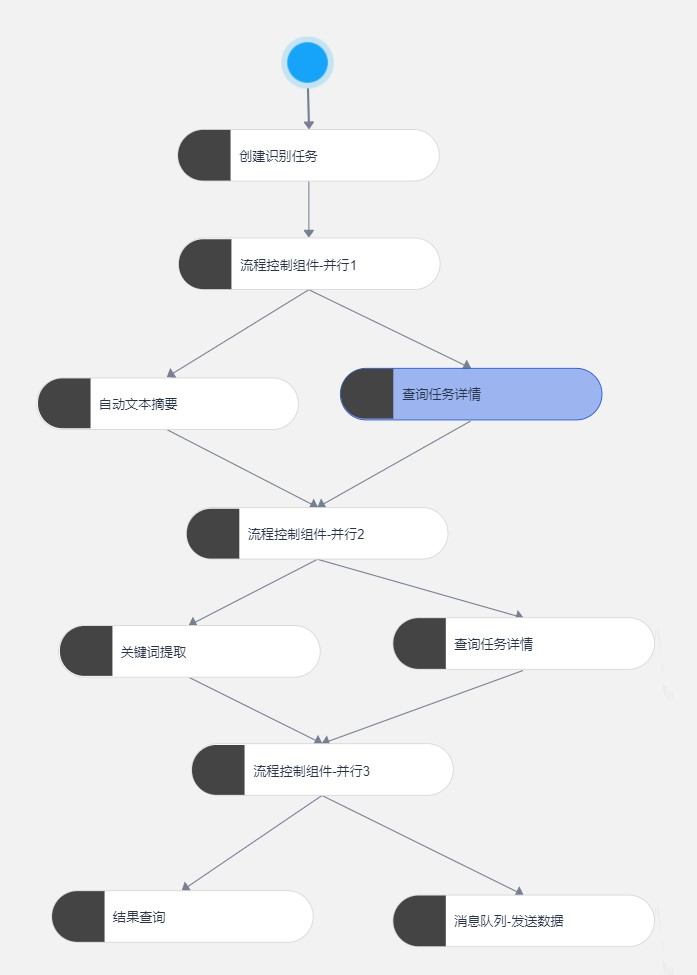
\includegraphics[width=0.7\textwidth]{3-3-2.jpg}
    \caption{编排应用实例}
    \label{fig:编排应用实例}
\end{figure}

如图2.1所示的实际应用场景,这是一个用户自定义编排给出的一个DAG输入,在该图给出的场景中,用户是定义了一个文本识别类的AI服务任务,只
有在用户显式指定了下游节点可以并行时,系统才会将这两个任务节点并行执行,而若没有显式指定,如“创建识别任务”和“流程控制组件-并行1”两
个节点就是串行执行的。而在实际工程当中,创建一个并行执行环境,要额外请求资源,这些资源的启动响应需要消耗时间,倘若能够用一种预测执
行器来提前预知这种情况,则可以在一开始就先请求这些资源,随后在执行整个服务时,就会消除该瓶颈,得到执行效率的提高。



\begin{figure}[H]
    \centering
    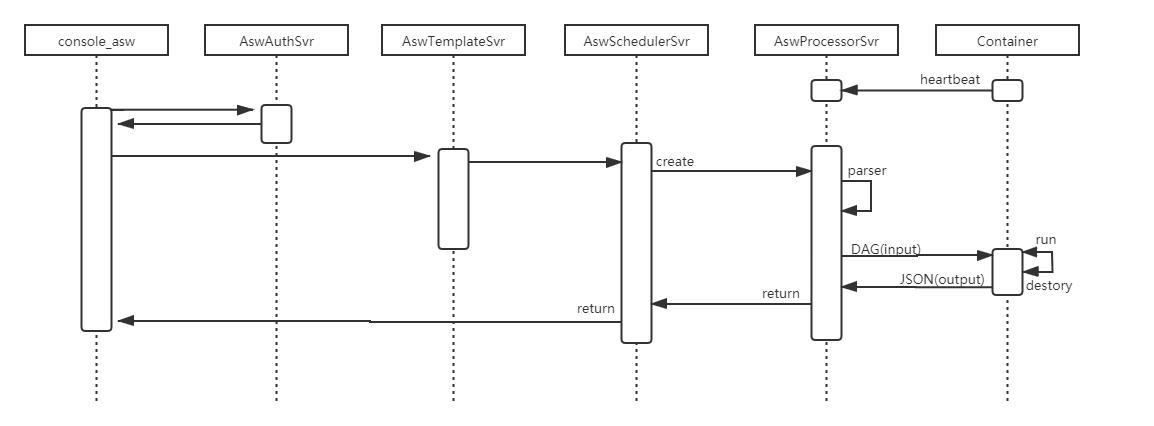
\includegraphics[width=0.9\textwidth]{3-2.jpg}
    \caption{普通执行器时序图}
    \label{fig:普通执行器时序图}
\end{figure}

如图2.2,用户视角的操作时序反映了整个服务被创建时的生命周期,也包含了整个系统的工作逻辑。用户通过JSON配置文件的方式在console发起一
次系统执行流程,用户的JSON会被解析为YAML表示的DAG,通过该YAML文件,顺序执行器AswProcessorSvr将会创建Container对象,并由执行器维
护对象的生命周期管理,顺序地执行每一个节点Node。

解析生成的DAG文件,每个结点会被乱序执行器分为两种类型,一种是无前置依赖的节点,与原逻辑同样的方式进行执行;大部分有前置依赖的节点,
将会使用分支预测的方式,预测最有可能的前置输入,交由容器执行。\cite{peng2021modelbased}

\begin{figure}[H]
    \centering
    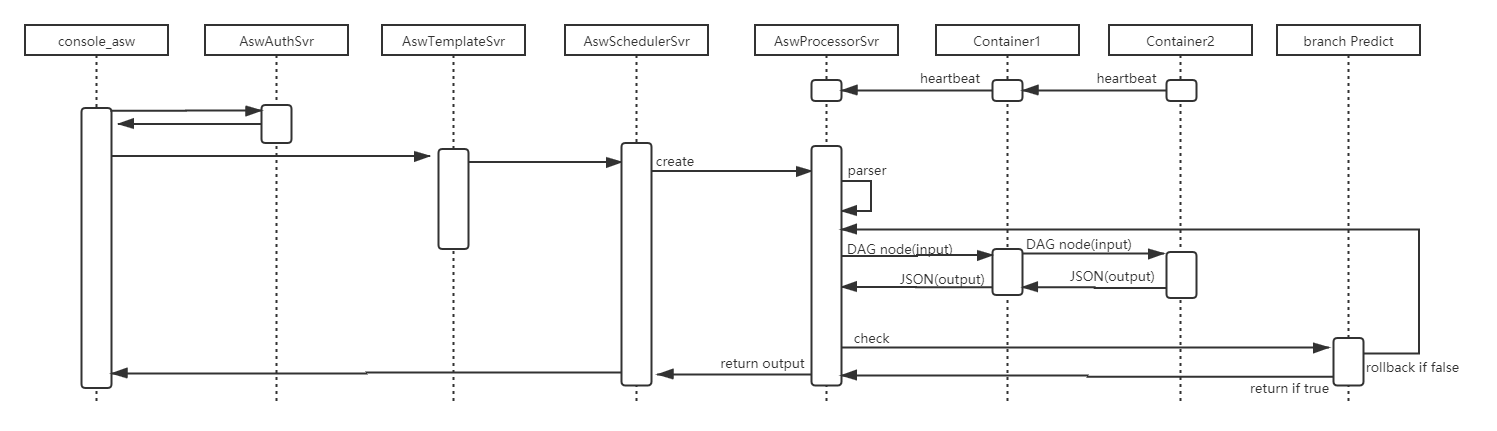
\includegraphics[width=0.9\textwidth]{3-3.jpg}
    \caption{并行执行器时序图}
    \label{fig:并行执行器时序图}
\end{figure}

图2.3对比图2.2,增设预测器,该部件负责提供节点根据历史执行记录信息统计得出的预测结果,先让执行器根据预测的结果将具体的工作流DAG发送
到调度器进行一次尝试执行,如果之后执行结果校验失败,调度器负责根据缓存器的结果进行重试,重新将任务执行发送到调度器。


\begin{figure}[H]
    \centering
    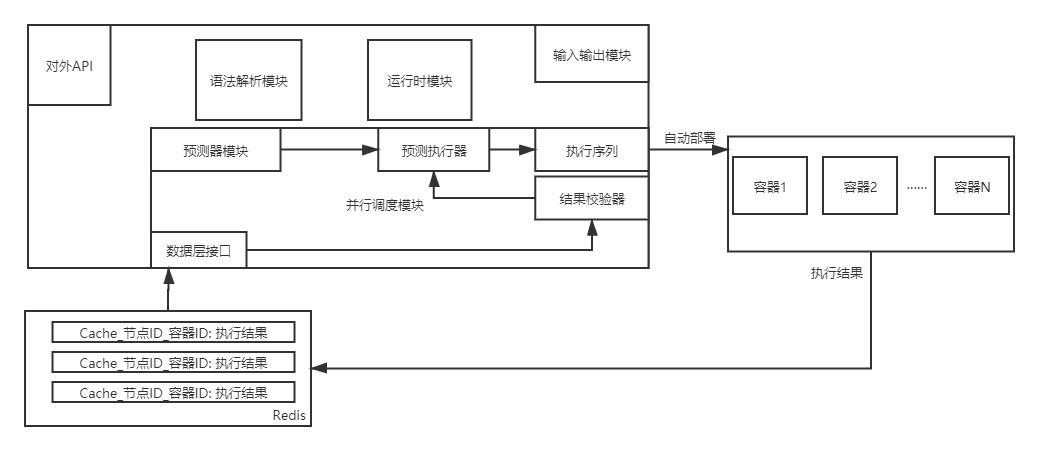
\includegraphics[width=1.0\textwidth]{4-1.png}
    \caption{模块架构}
    \label{fig:模块架构}
\end{figure}


如图4.1,执行器模块主要有如下部件:
\begin{itemize}
    \item 预测器:预测节点的输入输出,向并行执行器提出执行计划。设计思路借鉴指令重排序优化,根据历史执行记录,预测节点输入,如果碰到分支节点,
    则会预测最有可能执行的分支, 并向执行器申请资源完成执行,结果输出对其透明。该模块不负责保证预测结果的正确性,如果遇到预测失败,则会
    交由调度器负责从失败节点处开始转化为普通执行。
    \item 缓存器:辅助并行执行的部件,存储过程结果,不进行持久化。主要负责接收容器执行返回的结果,对没有及时返回结果的容器做阻塞处理,直到检测
    到容器销毁。存储的结果一定是已经执行完毕的。
    \item 并行执行器:由顺序执行器改进而来,区别是其需要和缓存器进行交互,根据缓存器提供的结果进行策略的选择。 主要功能与其相当,主要负责调度
    任务节点,建立节点与容器的逻辑关系,维持和容器的连接,向每个正在执行任务的容器检测心跳信号,对一定时间没有回复信号的节点做宕机标记处
    理,并负责重发给另外的容器执行任务。
    \item 语法解析器:提供基于状态机的DAG解析功能,是执行器模块的上游部件。
    \item 运行时模块:容器环境配置管理、容器心跳管理、容器动态注册管理。
    \item 结果校验器:负责保证结果的正确性,对不符合预期的执行条目做打回处理。该校验器的校验逻辑是不断检查当前缓存的执行结果是否有后续节点的条
    件不满足的情况发送,如果有,则代表包含此节点以后的所有执行都是不符合预期的,负责提出重新执行计划,回滚截止此节点之后的所有操作。

\end{itemize}

由于执行节点容易受到网络环境的影响,造成流量受阻或者完全不可用,因此需要实时监测执行节点容器的状态,执行器模块动态的负载状态检查职责如下:
在发送启动执行后, 执行器需要实时返回当前负载值,根据更新的负载值,动态更新执行节点容器的信息;定期探活获取负载值;
根据负载程度动态配置探活间隔, 任务多的时候, 频繁探活, 任务少的时候, 降低探活频率。


\subsection{鉴权微服务模块概要设计}

提供通用鉴权能力,对归类为敏感操作的业务流程进行行为控制。包括创建工作流资源,容器执行资源,执行预测,解析TCSL语言。实现思路如下图,
通过Gin框架的AOP能力,在处理中间件链前增加一个调用鉴权模块的Handler对象,输入带用户ID,工作流ID等信息的鉴权QRN字符串,返回一个具有
时效限制的Secret ID、Secret Key、Token,将这种行为成为“换票操作”。用于后续执行具体的业务流程的凭证,将该信息缓存于Redis,用户下次
调用会先判断缓存是否存在,无需短时间重复进行换票。

DescribeUserStatus:投递日志权限检查

\begin{figure}[H]
    \centering
    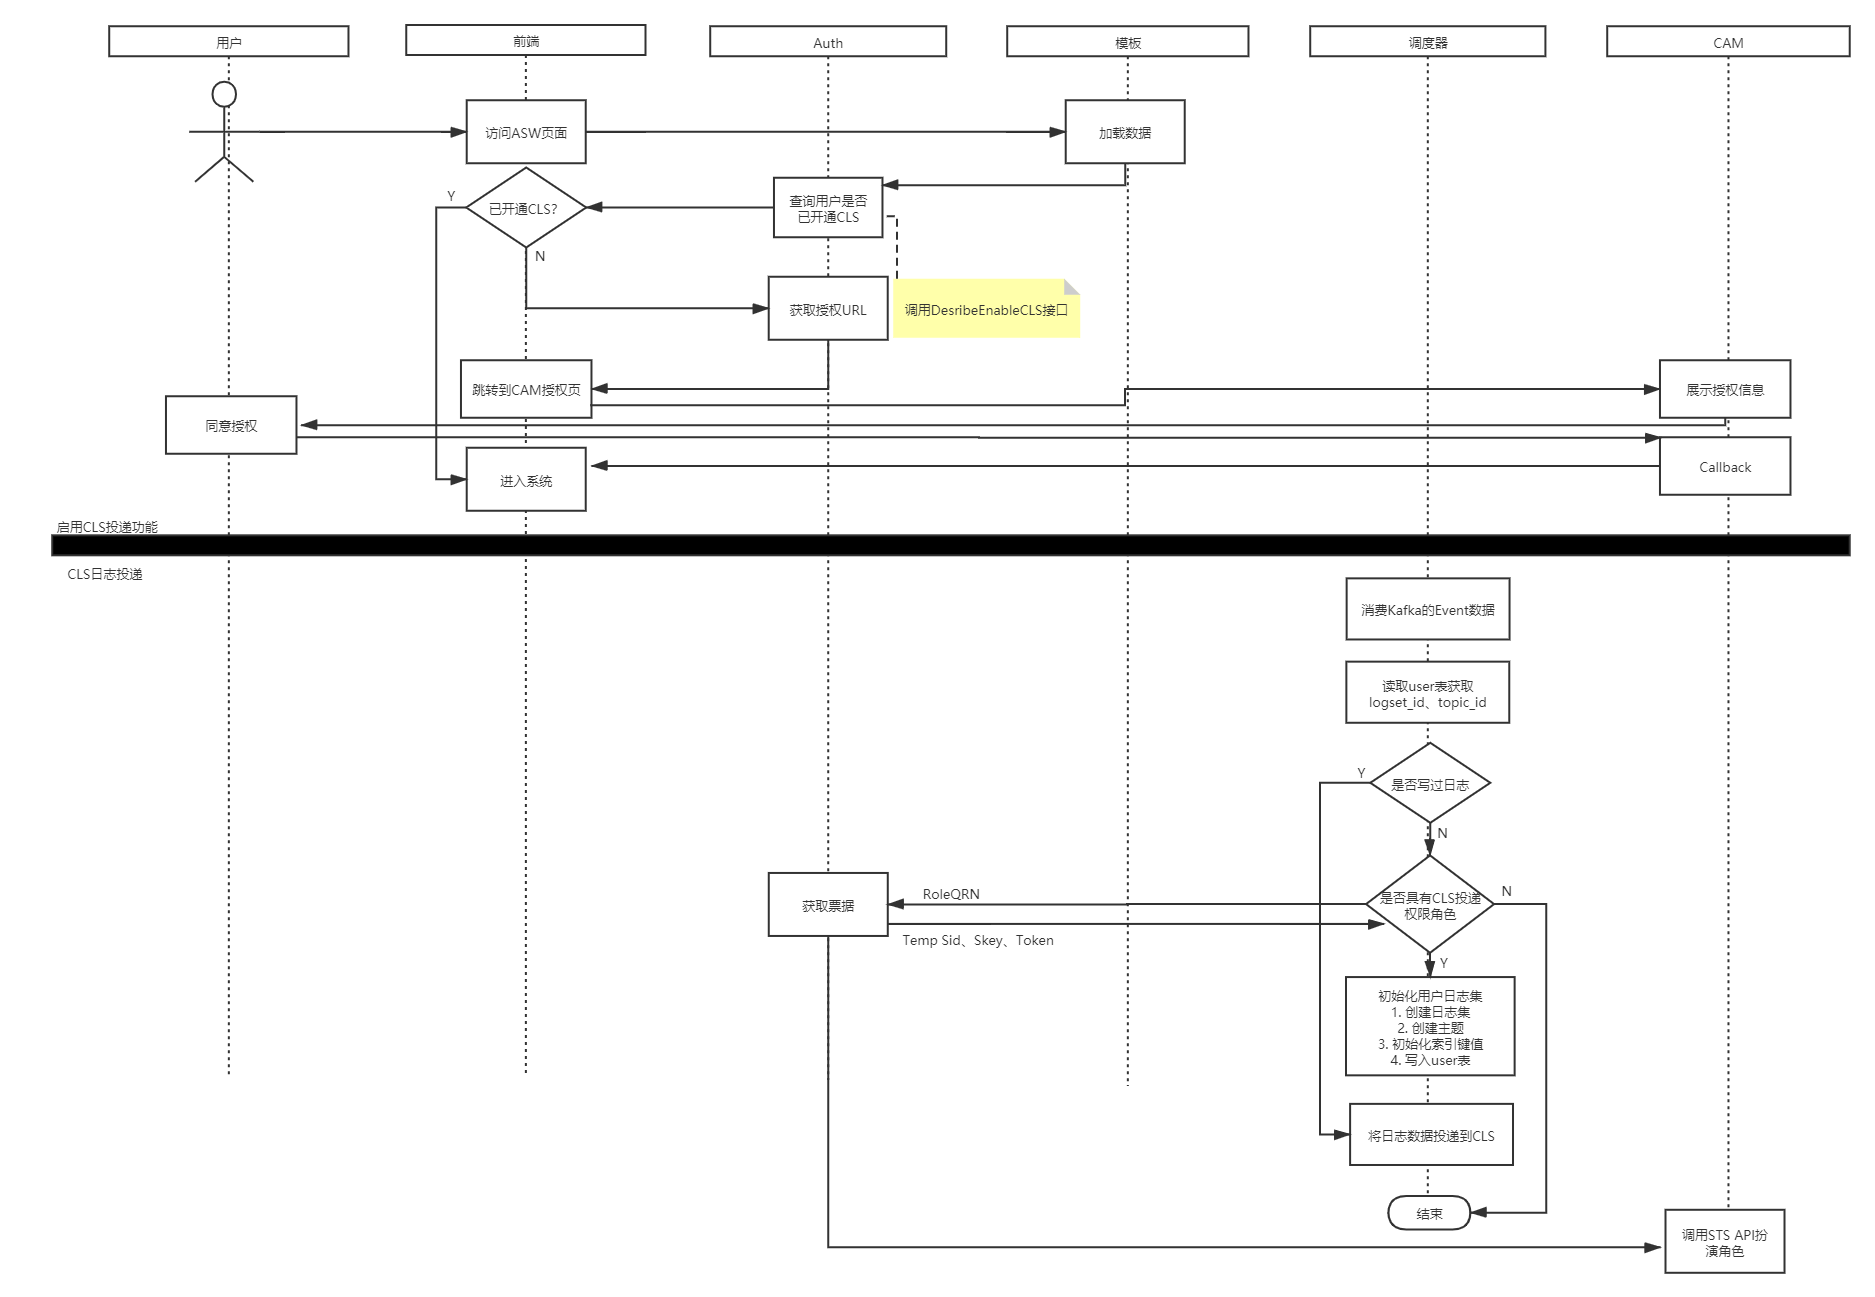
\includegraphics[width=0.9\textwidth]{cls-1.png}
    \caption{日志投递权限检查}
    \label{fig:rztdqx}
\end{figure}


\subsection{预测器服务模块}

\begin{figure}[H]
    \centering
    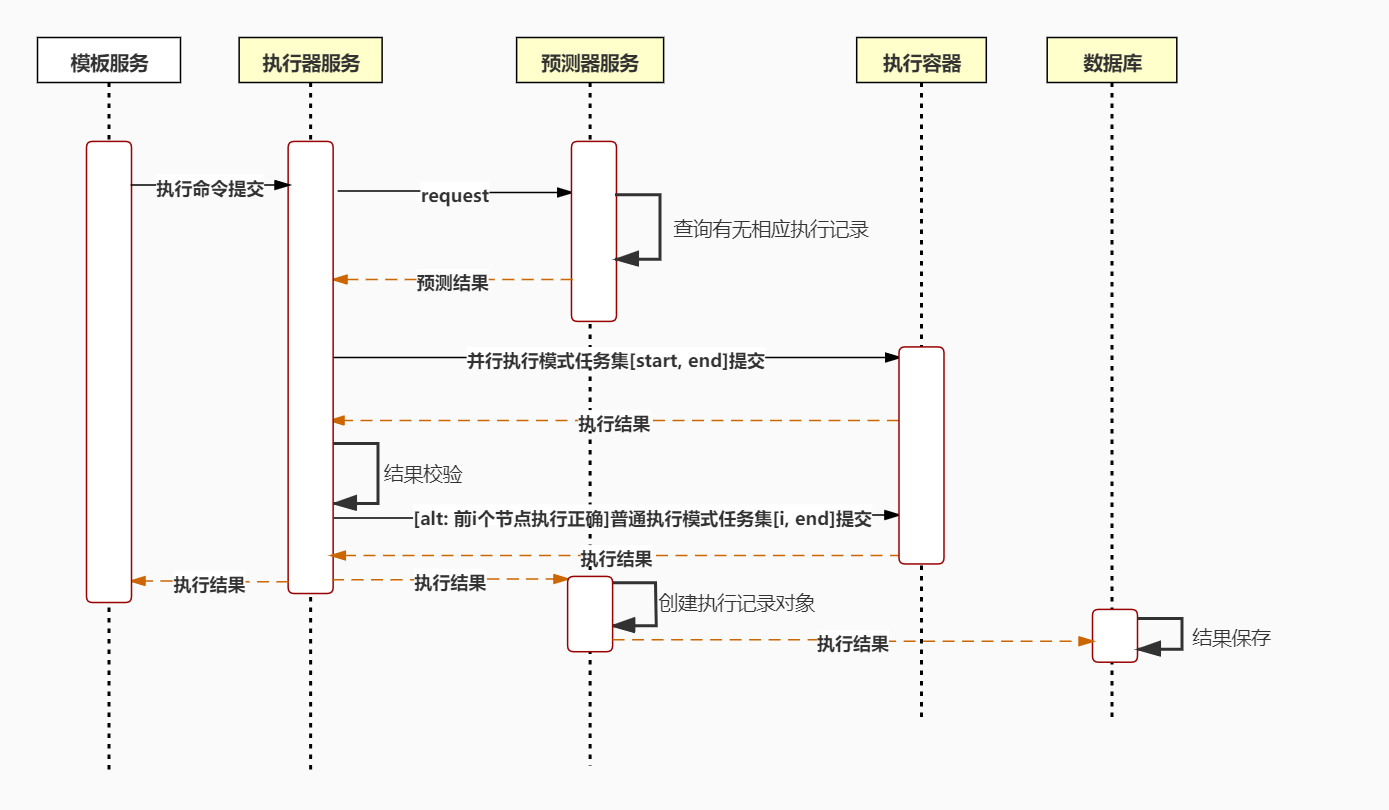
\includegraphics[width=1.0\textwidth]{sx_predict.jpg}
    \caption{预测器服务时序图}
    \label{fig:预测器服务时序图}
\end{figure}

如上图4.14所示,预测器主要负责提供执行结果记录、历史执行记录查询。为执行器模块直接提供服务。\cite{le2021deep}



\subsection{自动化测试方案设计}

\begin{figure}[H]
    \centering
    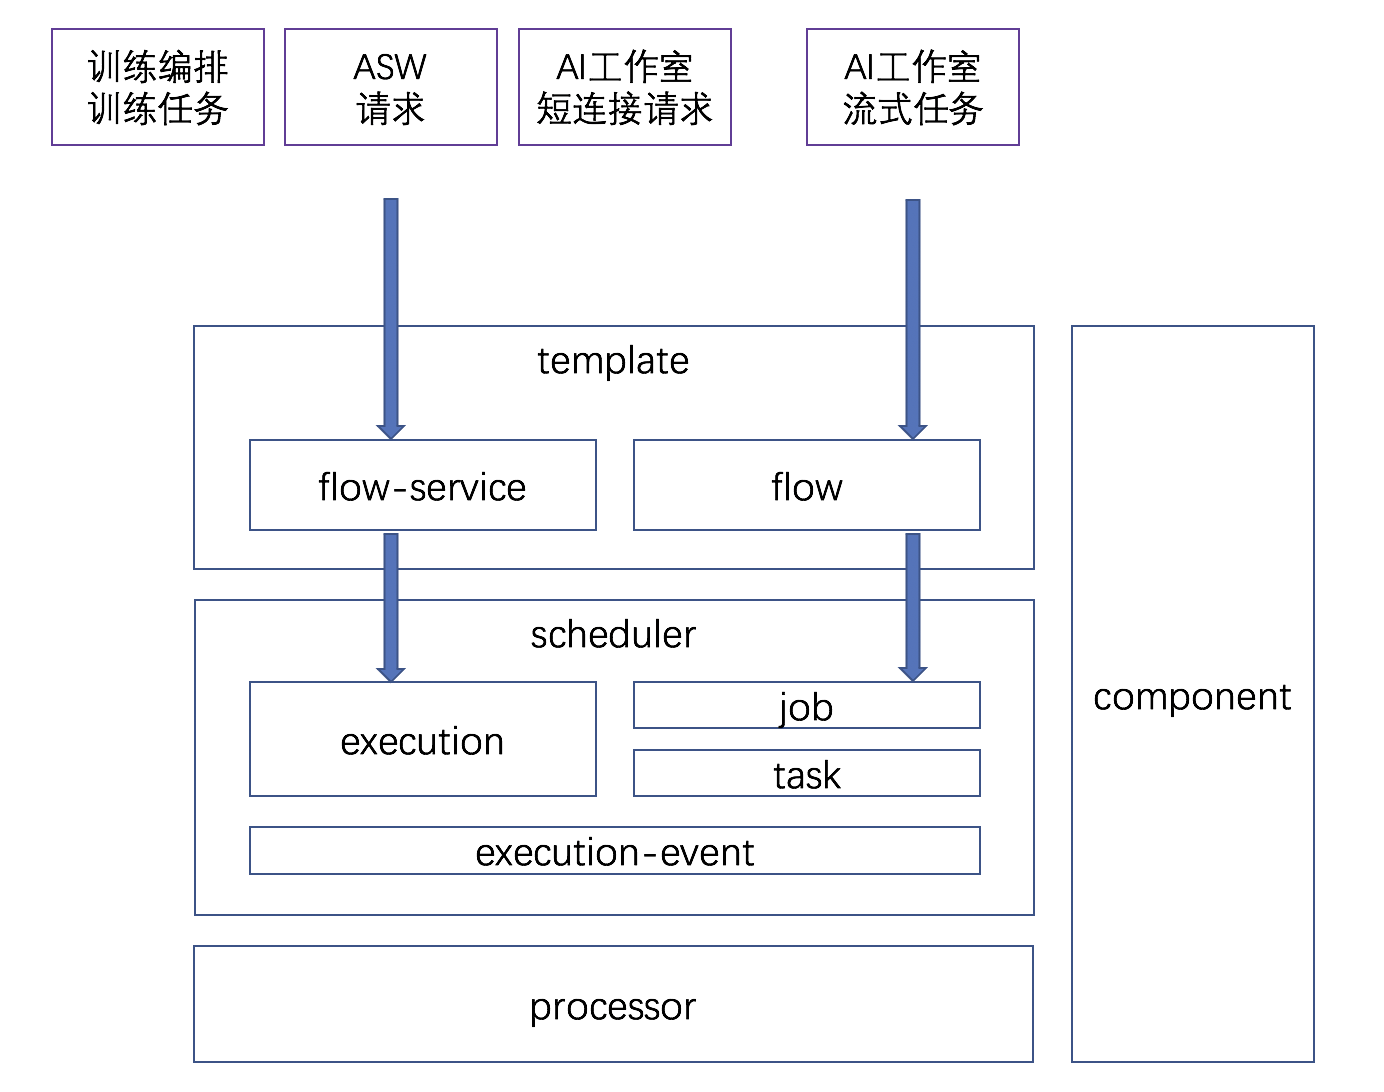
\includegraphics[width=1.0\textwidth]{asw-1.png}
    \caption{自动化测试流程}
    \label{fig:自动化测试流程}
\end{figure}



\subsubsection{自动化测试方案设计}

搭建测试工具包:
\begin{itemize}
    \item 使用sqlite3搭建mock数据库
    \item 使用migration-go, 进行数据库创建
    \item 使用xorm进行数据库操作(确保语法兼容)
    \item 使用jsonassert,进行json断言: https://github.com/kinbiko/jsonassert
\end{itemize}


二次开发jssonassert:
\begin{itemize}
    \item 结合https://github.com/Knetic/govaluate 对json中的内容进行语义解析
    \item 支持this > 10
    \item 支持this not empty
\end{itemize}


\subsection{日志巡检能力}

\begin{figure}[H]
    \centering
    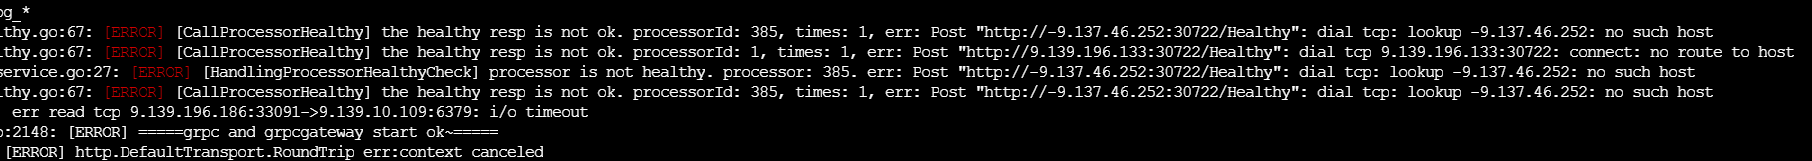
\includegraphics[width=1.0\textwidth]{log-3.png}
    \caption{日志巡检UML}
    \label{fig:日志巡检UML}
\end{figure}

\begin{enumerate}
    \item 取当前文件夹下所有*.log的文件,过滤出带[ERROR]的条目
    \item 排序,对每条ERROR日志通过编辑距离算法得到相似度,非常相似的日志不放入输出
    \item 输出每个log文件对应的error日志文件,以err\_log\_开头
    \item 输出search\_log\_run\_log文件是该脚本运行时的日志
\end{enumerate}

相似度计算代码如下。

\begin{algorithm}[H]
    \SetAlgoLined
    \KwData{sm,sn,threshold}
    \KwResult{1 - matrix[m-1][n-1] / max(len(sm), len(sn))}

    m,n = len(sm)+1,len(sn)+1

    matrix = [[0]*n for i in range(m)]

    matrix[0][0]=0

    for i in range(1,m):

    matrix[i][0] = matrix[i-1][0] + 1

    for j in range(1,n):

    matrix[0][j] = matrix[0][j-1]+1

    cost = 0

    for i in range(1,m):

    for j in range(1,n):

    if sm[i-1]==sn[j-1]:

    cost = 0

    else:

    cost = 1

    matrix[i][j]=min(matrix[i-1][j]+1,matrix[i][j-1]+1,matrix[i-1][j-1]+cost)

    Similarity = 1 - edit\_dist\_len / len(s)

\end{algorithm}

%\begin{algorithm}[h]
%    \SetAlgoLined
%    \KwData{this text}
%    \KwResult{how to write algorithm with \LaTeX2e }
%
%    initialization\;
%    \While{not at end of this document}{
%    read current\;
%    \eIf{understand}{
%    go to next section\;
%    current section becomes this one\;
%    }{
%    go back to the beginning of current section\;
%    }
%    }
%        \caption{算法示例1}
%        \label{algo:algorithm1}
%\end{algorithm}

\subsection{执行记录字典淘汰策略}
ZSet数据结构以时间序列来淘汰数据的策略: 通过一个独立的协程,定时调用清理逻辑,保持Redis中数据的总量不超过特定值。

%\begin{figure}[H]
%    \centering
%    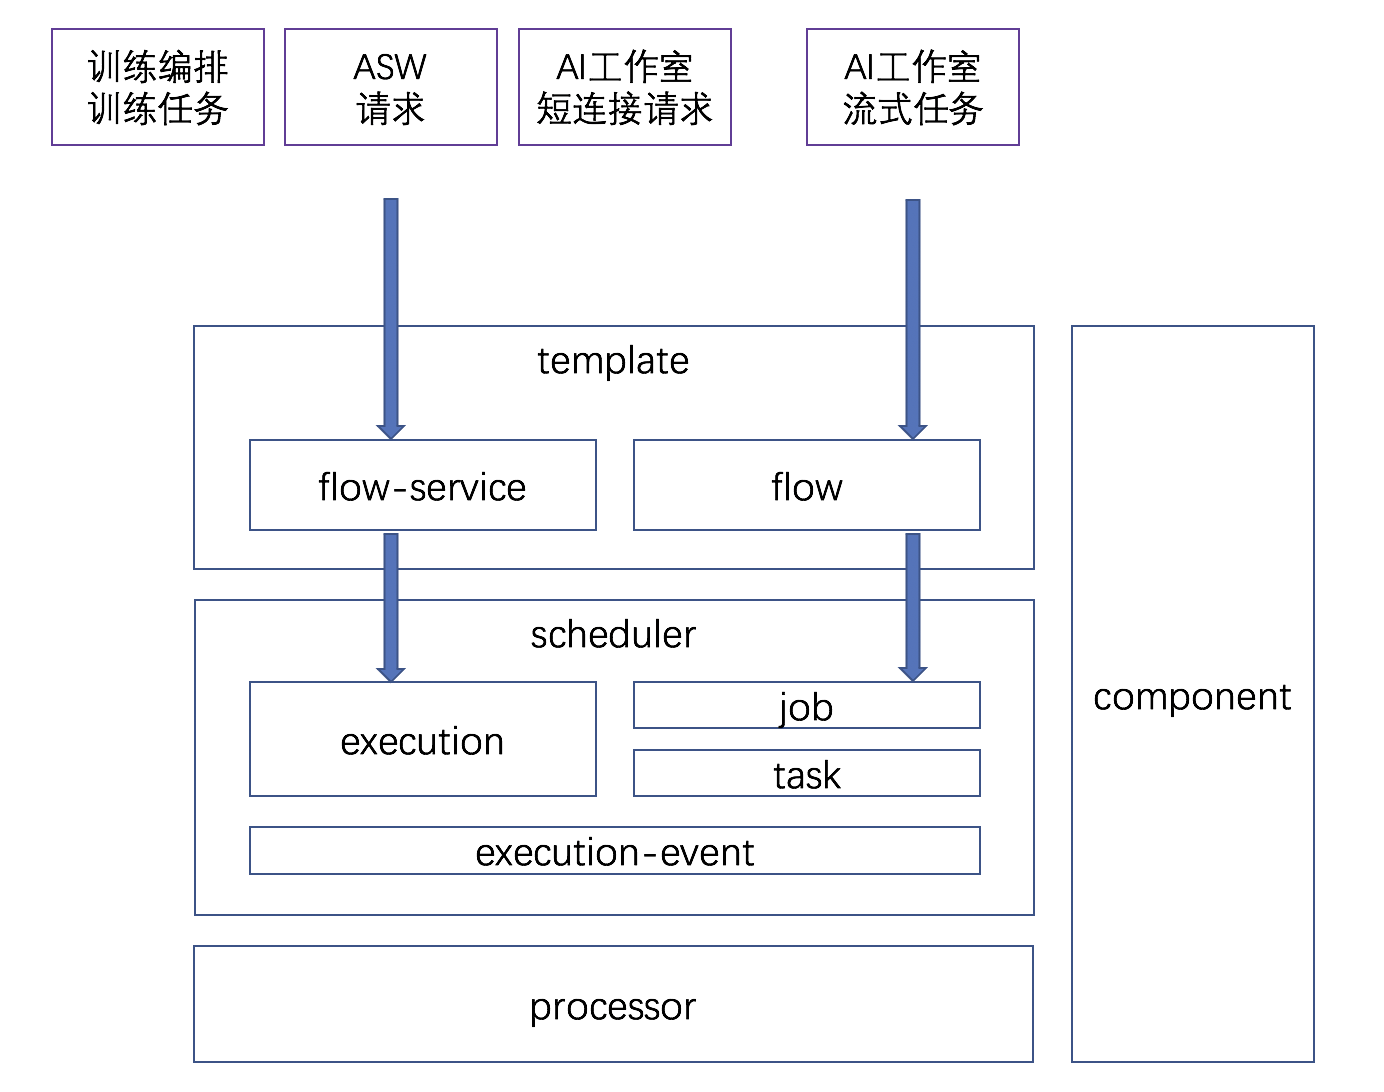
\includegraphics[width=1.0\textwidth]{asw-1.png}
%    \caption{淘汰策略UML}
%    \label{fig:淘汰策略UML}
%\end{figure}

这里采用主流的淘汰策略LRU(Least Recently Used): 即最近最少使用,是一种常用的页面置换算法,选择最近最久未使用的页面予以淘汰。该算法
赋予每个页面一个访问字段,用来记录一个页面自上次被访问以来所经历的时间t,当须淘汰一个页面时,选择现有页面中其t值最大的,即最近最少
使用的页面予以淘汰\cite{landman2021selfoptimizing}。

这也是Redis淘汰数据时采用的算法,但由于Redis不能按照时间序列来淘汰数据,仅支持设置指定日期Unix时间戳,设置内存占用大小阈值来淘汰,
因此,需要采用其它的方式来实现,实现代码如下。

\begin{algorithm}[H]
    \SetAlgoLined
    \KwData{scores}

    if len(scores) \> 0 \&\& len(scores)-1 \>= 0 \{

    firstScore := scores[0]

    lastScore := scores[len(scores)-1]
    deletedCount, err := executiondao.DeleteExecutionList(stateMachineQRN, firstScore, lastScore)

    if err != nil \{

    aswlogger.Errorf(nil, "[DeleteExecutionList] return error")

    \}

    aswlogger.Infof(nil, "last step deleteExecutionList done, delete count: \%d", deletedCount)

    \}
\end{algorithm}

\section{本章小节}
本章在需求分析的基础上,对该云服务的整体架构以及各个模块的设计进行详尽的阐述。阐述了现有方案存在的问题,以及优化的方案整体设计思路,
明确重点难点,有助于后续具体实现的工作进行。